
\chapter{Aufgabenblatt 03}


\section{Datenmodellierung}

\subsection{Aufgabe 1: ERM}

Ihnen liegt der nachfolgende Auszug aus dem Pflichtenheft vor. Bitte "uberf"uhren Sie diesen in ein Entity-Relationship-Diagramm mit Chen Notation.
Bestimmen Sie dazu die relevanten Entity-Typen, deren Beziehung untereinander soweie deren Kardinalit"aten und Attribute.
Bestimmen Sie daraufhin die jeweiligen Schl"usselattribute.\\

\noindent
\textbf{Auszug aus dem Pflichtenheft}
\begin{itemize}
    \item Jede Mensa ist eindeutig durch einen Namen, Ort und eine Dienststellennummer charakterisiert und wird durch einen Mensa-Chef geleitet.
    Dieser besitzt neben seinem Namen und Vornamen auch eine Personalnummer und einen Rang.
    Es kann auch m"oglich sein, dass der Chef f"ur mehr als eine Mensa Zust"andig ist.
    \item Jede Mensa bietet verschiedene Gerichte an.
    Es handelt sich dabei entweder um dauerhafte Angebote oder ein saisonales "`Special"'.
    Um die Zuordnung zu vereinfachen besitzt jedes der Gerichte eine interne Referenznummer, einen Namen und eine Beschreibung.
    Es kann sich dabei sowohl um eine Vor-, Haupt-, oder Nachspeise handeln.
    Die Gerichte haben dar"uber hinaus eine Bewertung, welche die Beliebtheit bei den Studenten widerspiegeln soll.
    Mede Mensa bietet zu unterschiedlichen Zeitpunkten unterschiedliche Gerichte an.
    \item Jedes der Gerichte besteht aus einer oder mehreren Zutaten.
    Diesen sind durch eine Bestelnummer und die Bezeichnung gekennzeichnet.
    Dar"uber hinaus dienen der Haltbarkeitszeitraum, die Angabe der m"oglichen Allergika sowie die Angabe ob vegetarisch oder nicht als wichtige Informationen.
\end{itemize}

\bigskip
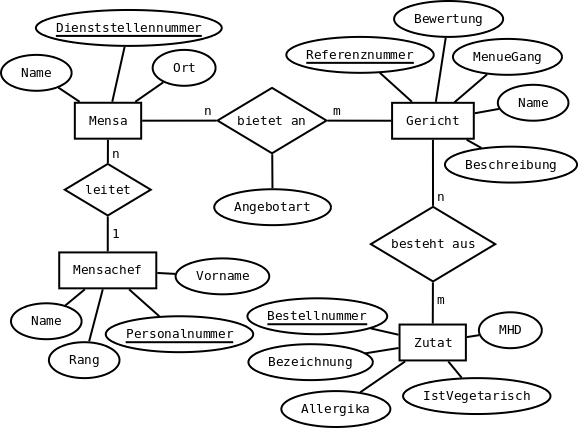
\includegraphics[scale=0.5]{./inc/aufgabe03/mensaapp.png}

\subsection{Aufgabe 2: Relationenschema}
"Uberf"uhren Sie nun das von Ihnen erstelte ERM-Diagramm in das Relationenmodell.\\

\noindent
\fbox{
    \parbox{\textwidth}{
        \textbf{Mensachef}(\underline{Personalnummer}, Name, Vorname, Rang)\\
        \textbf{Mensa}(\underline{Dienststellennummer, Name, Ort}, $\overline{Personalnummer}$)\\
        \textbf{Gericht}(\underline{Referenznummer}, Name, Beschreibung, MenueGang, Bewertung)\\
        \textbf{Zutat}(\underline{Bestellnummer}, Bezeichnung, MHD, Allergika, IstVegetarisch)\\
        \textbf{Rezept}(\underline{GerichtId[Gericht], ZutatId[Zutat]})\\
        \textbf{Speiseplan}(\underline{GerichtId[Gericht], MensaId[Mensa]}, Angebotart)\\
        
        \noindent
        {\small \textbf{Anm. des Autors}: Fremdschl"usselbeziehungen k"onnen entweder durch einen Oberstrich gekennzeichnet werden, oder durch das Angeben der Tabelle, auf die der  Fremdschl"ussel refenziert, in eckigen Klammern.\\
        Im Zweifel sollte w"ahrend der Klausur die Methode der Vorlesung gew"ahlt werden!}
    }
}







